This chapter discusses the relevance of \bpfbox{} and \bpfcontain{}, positioning them as
novel extensions on top of the existing confinement literature. We also examine
limitations of both research systems and present opportunities for future work. Namely, we
propose ways to address current limitations, improve the \gls{ebpf} ecosystem for
confinement use cases, add features to \bpfbox{} and \bpfcontain{}, and conduct further
research on the usability of both systems.

% \begin{inprogress}
%   New planned outline:
%   \begin{itemize}
%     \item 8.1 Contributions
%     \begin{itemize}
%       \item A paragraph per chapter (starting with 3), 1--2 sentences per section,
%             outlining the key points of what I did
%     \end{itemize}
%     \item 8.2 Limitations
%     \begin{itemize}
%       \item Leave this mostly unchanged
%       \item But revisit the \enquote{passive overhead} section (possibly remove BPF
%       namespaces part, depending on if we decide to keep it in)
%     \end{itemize}
%     \item 8.3 Future Work and Research Directions
%     \begin{itemize}
%       \item Keep policy language experimentation and user study
%       \item Possibly remove \gls{bpf} namespace and unprivileged \gls{bpf}?
%       \item Keep Docker integration and OCI spec
%       \item Keep fine-grained network policy
%       \item Remove GUI, keep policy generation
%     \end{itemize}
%     \item 8.4 Conclusion
%     \begin{itemize}
%       \item Leave this as-is and maybe fold in some of the pontificating from
%             \enquote{Improving the Status Quo}
%     \end{itemize}
%   \end{itemize}
% \end{inprogress}

\section{Contributions}%
\label{s:disc-contributions}

In \Cref{c:confinement-problem}, we presented a novel framing of the confinement problem,
arguing that inherent complexities in Linux confinement can be solved with the
introduction of simple, unified mechanisms designed for process- and container-level
confinement. We also argue that there is no fundamental reason why containers cannot be
considered as secure as virtual machines, since a container expose specific interfaces to
the outside world, just as a virtual machine does. We identify fundamental issues with
Linux confinement, highlighting its complexity, unsuitability for containers, and the poor
adoptability of alternative solutions. We also examine how container frameworks apply
confinement primitives and discuss the fundamental reasons underlying their fail-open
approach to security. In light of this analysis, we outline the design goals for \bpfbox{}
and \bpfcontain{}, explain how the latter evolved from the former, and present a threat
model for confinement.

In \Cref{c:bpfbox}, we outline the design and implementation details of \bpfbox{},
a proof-of-concept sandboxing framework based on \gls{ebpf} programs attached to \gls{lsm}
hooks.  We provide an overview of \bpfbox{}'s design and explain how policy enforcement
works at a high level. \bpfbox{} translates policies written in a simple, domain-specific
language into entries in \gls{ebpf} maps, then resolves policy at runtime using \gls{ebpf}
programs attached to \gls{lsm} hooks. We then discuss the specific implementation details
of \bpfbox{}'s enforcement engine and document an early version of its policy language.

In \Cref{c:bpfcontain}, we describe the design and implementation of \bpfcontain{},
a successor to \bpfbox{} that focuses on container-level confinement. We highlight
\bpfbox{}'s limitations and describe how \bpfcontain{} improves upon the original
\bpfbox{} design. Specifically, \bpfcontain{} eliminates large dependency overheads,
enabling it to be compiled once and run on any supported target kernel. \bpfcontain{} also
introduces container semantics into its enforcement engine design and simplifies and
extends \bpfbox{}'s policy language. We provide an overview of \bpfcontain{}'s design and
explain how it enforces policy at a high level. We then describe \bpfcontain{}'s specific
implementation details and document the schema of its policy language, focusing on
policies written in the YAML serialization format.  We also describe how a future
iteration on \bpfcontain{} can integrate with Docker, introducing additional container-level
semantics that can simplify policies.

In \Cref{c:evaluation}, we present an evaluation of \bpfbox{} and \bpfcontain{} in terms
of their performance overhead and security. Specifically, we conduct a series of micro-
and macro-benchmarking tests comparing \bpfbox{} and \bpfcontain{} with the base system
and AppArmor, a popular \gls{lsm}. We find that \bpfbox{} and \bpfcontain{} perform
competitively with AppArmor in the macro-benchmarks, despite being unoptimized research
prototypes. We also present a detailed security analysis of \bpfbox{} and \bpfcontain{}
pointing out potential weaknesses in policy enforcement and describing how they can be
rectified.

In \Cref{c:case-studies}, we present example policies for \bpfbox{} and \bpfcontain{},
targeting three realistic use cases. We first examine how \bpfbox{} and \bpfcontain{} can
be used to confine a simple Apache httpd and mysqld deployment. We then consider how
\bpfbox{} and \bpfcontain{} can be used to implement Docker's default confinement policy,
and finally examine how a future version of \bpfcontain{} can be used to secure an
untrusted Docker container with minimal effort.

\section{Limitations}%
\label{s:disc-limitations}

In this section, we discuss some limitations of the \bpfbox{} and \bpfcontain{}
prototypes. While some limitations arise due to a lack of support for the correct
primitives in the current \gls{ebpf} ecosystem, others arise due to the prototypical
nature of \bpfbox{} and \bpfcontain{} as research systems. In both cases, we discuss how
future iterations of \bpfbox{} and \bpfcontain{} can address these limitations, either
through extensions to the policy enforcement mechanism or future improvements to the
\gls{ebpf} ecosystem.

%\subsection{Limited Pathname Support in \glsentryshort{ebpf}}
\subsection{Semantic Issues in the Policy Language}%
\label{ss:disc-semantic-issues}

It is hard to refer to files from \gls{ebpf}. In the kernel, files are generally uniquely
described by an \textit{inode} structure, which in turn maps to one or more pathnames via
a \textit{file} structure. Each inode belongs to a distinct filesystem, and is uniquely
enumerated within that filesystem by an inode number.  In \bpfbox{} and \bpfcontain{}, we
uniquely identify inodes using a combination of their inode number and the unique device
identifier of the filesystem on which the inode resides. While this is an effective
technique for runtime monitoring, things begin to fall apart when dealing with
a \textit{user-facing} data store, such as a policy map.

While the kernel refers to files by their inodes within a filesystem, users do not. For
the most part, userspace does not deal in inode-level semantics\,---\,instead, we deal in
\textit{pathnames}, a string that describes the path required to move from the filesystem
root to a given file. Indeed, the \bpfbox{} and \bpfcontain{} policy languages use
pathnames rather than inodes to refer to files. Unfortunately, this creates an undesired
dichotomy between the user-facing components of \bpfbox{} and \bpfcontain{}, and the
kernelspace implementation.  To resolve this dichotomy, we translate the pathnames into
inode and device pairs at policy load-time. This is a workaround and is subject to several
fundamental limitations. In particular, referring to a pathname that doesn't yet exist
becomes difficult, as inode numbers do not yet exist; inodes that are deleted or freshly
created at runtime must be treated as special cases, dynamically updating the policy as
required; finally, globbing pathnames can result in an explosion in the size of maps
storing file rules, as each globbed file is translated into a unique inode-device pair.

To resolve these issues, it would be ideal if we could refer to pathnames directly from
\gls{bpf} programs. In particular, a design using this capability might resolve pathnames
within \gls{ebpf} programs and define a finite state machine to match globbing rules over
the pathname. Unfortunately, current support for pathname resolution in \gls{ebpf} is primitive.
Difficulties arise due to a few fundamental limitations imposed by the verifier and the \gls{ebpf}
runtime:
\begin{enumerate}
  \item The verifier imposes a hard limit of 512 bytes of stack space for each \gls{bpf}
  program. This makes it unrealistic to store strings on the stack, instead requiring that
  a buffer be allocated in the heap. In the context of \gls{bpf}, this can only be done
  using a dummy map as a scratch buffer.

  \item The verifier also imposes restrictions on how \gls{ebpf} programs can loop and how
  these loops can access map data. Specifically, loops must provably terminate and any
  array access within a loop must be appropriately bounded by a fixed constant (to ensure
  no buffer overflows or similar issues). In practice, enforcing these restrictions is
  difficult, and the verifier errs on the side caution when reasoning about a loop is unclear.
  This can result in safe programs that manipulate long strings being erroneously rejected.

  \item While helper functions can get around such restrictions, the current ecosystem for
  string manipulation helpers in \gls{ebpf} is immature. For instance, Linux 5.10 added
  a \texttt{bpf\_d\_path()} helper~\cite{olsa2020_d_path} to extract pathnames from
  a kernel directory entry. However, this helper is only available for sleepable \gls{bpf}
  programs, since allocating a buffer for the string can result in a page fault. Support
  for sleepable \gls{bpf} is very new and has not had a chance to mature; currently,
  sleepable programs are restricted to a small subset of \gls{lsm} programs. Aside from
  pathname resolution, no other string helpers currently exist, although they have been on
  the radar of \gls{ebpf} developers for some time.
\end{enumerate}

Although the current state of the \gls{ebpf} ecosystem makes it impossible for \bpfbox{}
and \bpfcontain{} to directly use pathname-based enforcement in the kernel, this will not
necessarily be the case in the future. \gls{ebpf} is in active development, and each
subsequent kernel version adds new features and capabilities. For instance, the kernel
community is currently working on a generic solution for sleepable \gls{bpf} that will
greatly expand the number of programs that can handle page faults. When this support
arrives, it is likely that working with strings will become much easier. Thus, future
versions of \bpfbox{} and \bpfcontain{} will likely be able to incorporate pathname-based
policy enforcement in their kernelspace implementations.

% \begin{inprogress}
%   \begin{itemize}
%     \item Hard to refer to files from \gls{ebpf}
%     \item Currently, \bpfbox{} and \bpfcontain{} translate file policy into inodes and filesystem device IDs
%     \item This is a crude workaround; it has some convenient side effects for security,
%     but issues arise when we want to refer to pathnames that don't exist yet
%     \item It can also cause an explosion in the size of maps storing file rules, as
%     globbed paths get translated into multiple rules: one for each file that matches the
%     glob

%     \item The difficulty working with pathnames is partially a result of a fundamental limitation of \gls{ebpf}: difficulty manipulating strings
%     \item Problem generally arises from three factors, primarily related to the verifier:
%     \begin{itemize}
%       \item Verifier imposes a hard 512 byte limit on stack allocations (strings need to be heap-allocated, stored in an map)
%       \item Verifier imposes restrictions on how programs can loop (looping needs to provably terminate, the verifier errs on the side of caution here)
%       \item Helper functions can get around these restrictions, but decent string and pathname helpers are no here yet
%     \end{itemize}
%     \item Another fundamental issue is that support for sleepable \gls{bpf} is new and has
%     not yet matured (only a small subset of \gls{lsm} programs can currently be marked
%     sleepable)
%     \item Linux 5.(11?) added \texttt{bpf\_d\_path}, but this is only callable from sleepable programs, a subset of \gls{lsm} programs
%     \item In the current \bpfbox{} and \bpfcontain{} design, this limitation is too restrictive
%     \item Luckily, it seems like the community is working towards a general solution to
%     this problem (dynamic map allocation and making more program types sleepable)
%     \item As the \gls{ebpf} ecosystem evolves, it may be possible to support pathnames as
%     a first class citizen, removing the requirement for working with inodes and filesystem
%     numbers
%   \end{itemize}
% \end{inprogress}

\subsection{Fixed-Size Policy Maps}

Currently, policy maps under \bpfbox{} and \bpfcontain{} are of a fixed size, determined
at policy load time. This is due to a fundamental limitation of \gls{ebpf}: maps must be
allocated at a fixed size and may not be directly resized at runtime. To get around this
limitation, \bpfbox{} and \bpfcontain{} tailor policy map size to the number of rules that
will be loaded into the kernel. While this approach is effective, it would be better to
have the ability to dynamically grow policy maps at runtime. This would enable \bpfbox{}
and \bpfcontain{} to support loading arbitrary length policies at runtime, and even
runtime policy generation, without over-fitting map sizes.

As with string helpers in the previous section, the primary bottleneck preventing
dynamically-sized maps is the adoption of sleepable \gls{bpf}. Alexei Starovoitov expects
that subsequent versions of the kernel will support dynamically allocated maps as the
number of sleepable \gls{bpf} programs increases. When support for this lands, \bpfbox{}
and \bpfcontain{} will be able to leverage this new functionality to greatly improve the
memory efficiency of policy maps and support runtime policy generation from the \gls{ebpf}
side.

% \begin{inprogress}
%   \begin{itemize}
%     \item Currently, policy maps are of a fixed size
%     \item It's okay to make them big, since \gls{ebpf} does support map growth up to a fixed limit
%     \item But we are still limited in total map size (todo: get current figure)
%     \item In our current implementation, we simply grow policy maps from userspace when the map size would be too small to fit current rules
%     \item But this approach is still limited, as it doesn't support map resizing at runtime, only at load time
%     \item Once sleepable \gls{bpf} matures, we can have dynamically allocated maps of
%     arbitrary size at runtime (link Alexei's LKML thread), as we can now have runtime map
%     allocators where is it okay to sleep on a page fault
%   \end{itemize}
% \end{inprogress}

% \subsection{Passive Performance Overhead}

% According to the performance evaluation results in \Cref{s:eval-performance} of
% \Cref{c:evaluation}, both \bpfbox{} and \bpfcontain{} offer competitive performance with
% AppArmor while offering the higher flexibility afforded to an \gls{ebpf}-based
% implementation. While these results are satisfactory, based on the number of additional
% benefits these research systems provide, there is a key opportunity to improve performance
% in one critical area: passive overhead on the system as a whole. \todo{We are in SELinux
% territory, we are playing the same game they are... It's already what everyone uses, so
% overhead being in line is acceptable}

% The problem is as follows. \bpfbox{} and \bpfcontain{} are designed to be process- and
% container-specific, rather than enforcing policy globally. Thus, they would ideally exert
% no additional performance overhead on unconfined applications. However, \gls{ebpf} and the
% \gls{lsm} hooks themselves are both \textit{global} mechanisms. Whenever a process make
% a system call, it always triggers the corresponding \gls{lsm} hook, which in turn always
% triggers the corresponding \gls{bpf} program. To filter out unconfined processes, we use
% a simple map lookup to query the process state\,---\,if it exists, we assume a confined
% process; if not, we assume an unconfined process and return early. Item \Circled{A} in
% \Cref{fig:disc-hooks} depicts this code path.

% Ideally, we would like to implement a filter that triggers \textit{before} \gls{lsm} hook
% invocation. Item \Circled{B} in \Cref{fig:disc-hooks} depicts this alternative code path.
% By filtering early, we could avoid the overhead of dynamic dispatch into the \gls{lsm}
% hook and \gls{bpf} program invocation entirely in the passive case. Thus, such an
% implementation would significantly outperform traditional \glspl{lsm} such as AppArmor and
% SELinux in global overhead, at a slight fixed cost of invoking filter logic before hook
% invocation.  Intuitively, it makes sense that the current \gls{lsm} hooks implementation does
% not employ this strategy\,---\,classically, \gls{lsm} hooks were \textit{meant to be global}.
% With the advent of the \gls{bpf} \gls{lsm}, this is no longer necessarily the case.

% \begin{figure}[htpb]
%   \centering
%   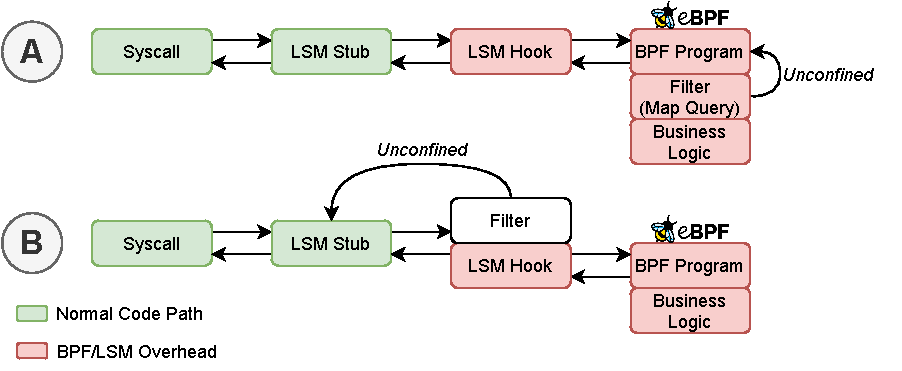
\includegraphics[width=0.8\linewidth]{figs/discussion/hooks.pdf}
%   \caption[The code path taken by BPF LSM and accompanying overhead]{
%     The code path taken by \gls{bpf} \gls{lsm} and accompanying overhead. \Circled{A} shows the current \gls{bpf}
%     \gls{lsm} implementation. System calls invoke \gls{lsm} stubs which trigger dynamic
%     dispatch into \gls{lsm} hooks. These hooks then invoke a \gls{bpf} program, which
%     implements filtering and security enforcement logic. \Circled{B} shows the ideal
%     implementation that optimizes for overhead in the passive case by filtering
%     \textit{before} \gls{lsm} hook invocation.
%   }%
%   \label{fig:disc-hooks}
% \end{figure}

% Transitioning from the existing \gls{lsm} execution model to the model proposed above will
% require explicit support from the kernel. Since it likely does not make sense to offer
% such filtration logic in the general case, any implementation will likely need to be
% \gls{bpf}-specific. \Cref{ss:bpf-namespace} proposes a realistic extension to the
% \gls{bpf} ecosystem that could make such a change feasible: the \gls{bpf} namespace.

% \begin{inprogress}
%   \begin{itemize}
%     \item Currently, \bpfbox{} and \bpfcontain{} are competitive with mainstream
%     confinement solutions based on \gls{lsm} (e.g.~AppArmor, see chapter 6)
%     \item This competitiveness is actually an advantage, considering that \bpfbox{} and
%     \bpfcontain{} can be dynamically loaded and attached to various system events. In this sense,
%     we are getting increased flexibility without paying much of a cost in performance.
%     \item But, \bpfbox{} and \bpfcontain{} have the potential to be far more performant than
%     conventional \gls{lsm}s in one critical case: passive overhead on the rest of the system.
%     \item Due to a current limitation of how KRSI works, its \gls{ebpf} \gls{lsm} hooks are
%     always globally invoked, regardless of whether the target process is of interest to us or not.
%     \item The current pattern looks like (Invoke Syscall $\rightarrow$ Invoke Hook
%     $\rightarrow$ Invoke BPF Program $\rightarrow$ Filter Logic $\rightarrow$ Return from
%     BPF Program $\rightarrow$ Return from Hook $\rightarrow$ Return from Syscall).
%     \item In the future, we may be able to move the filter logic to the step
%     \textit{before}  the hook is called, or at the very least before the BPF program is
%     called. This would nearly eliminate any passive overhead on the unconfined parts of the system.
%     \item I have a plan for this: introducing a new namespace for \gls{bpf} programs and
%     maps. (Forward ref to BPF namespace and unprivileged BPF)
%   \end{itemize}
% \end{inprogress}

\subsection{Performance Overhead}

The performance results presented in \Cref{c:evaluation} indicate that \bpfbox{} and
\bpfcontain{} have higher overhead than AppArmor in the OSBench micro-benchmarks.
However, this is not indicative of their performance in the general case. In fact,
\bpfbox{} and \bpfcontain{} perform competitively with AppArmor in the macro-benchmarks,
suggesting that the overhead of individual system calls is outweighed by the computational
complexity of an instrumented application and the synchronous delays introduced by
blocking system calls on I/O. Moreover, neither \bpfbox{} nor \bpfcontain{} has been
deliberately optimized, suggesting that there may be opportunities to improve performance
in the future.

In addition to considering potential improvements to their base overhead, we must also
consider the additional flexibility provided by an \gls{ebpf}-based confinement mechanism.
Using \gls{bpf} \gls{core}, \bpfcontain{} can be run on any supported kernel without the
need to recompile or patch either the kernel of \bpfcontain{} itself. The dynamic nature
of \gls{ebpf} means that software bugs or vulnerabilities in the enforcement engine can be
fixed without the need to update the kernel or even reboot the system. Moreover,
\gls{ebpf} programs are verified for safety, meaning that they are far less likely to
expose additional attack surfaces in the kernel than a kernel patch or loadable kernel
module.

% \begin{inprogress}
%   \begin{itemize}
%     \item \bpfbox{} and \bpfcontain{} have higher overhead in the micro-benchmarks
%     \item The overhead averages out in the general case
%     \item And they perform competitively with AppArmor in the macro-benchmarks, suggesting
%           that the overhead of individual operations is outweighed by computational complexity
%           and the synchronicity of blocking system calls
%     \item Also, what we are buying for the additional overhead is increased flexibility
%     \item Unlike a traditional \gls{lsm}, an \gls{ebpf}-based confinement mechanism can be
%           plugged into any supported kernel and just work. Moreover, any bugs or design flaws
%           that crop up in an \gls{ebpf}-based implementation can be patched without updating the
%           kernel, similar to how we update userspace programs.
%   \end{itemize}
% \end{inprogress}

% Both exhibit higher performance overhead than AppArmor in many of
% the micro-benchmarks presented . While the performance results in \Cref{c:evaluation} do show
% that \bpfbox{} and \bpfcontain{} are competitive with AppArmor in the macro-benchmarks and that
% they beat AppArmor in worst-case overhead,

% \todo{Talk about how we are a bit higher overhead, but we get so much more flexibility}
% \todo{The overhead is not that bad, and it's not an optimized thing. This can be improved with more optimizations.}

\subsection{Security Guarantees}

In \Cref{c:evaluation}, we presented a detailed security analysis of the \bpfbox{} and
\bpfcontain{} designs.  However, this informal analysis is weak evidence for the actual
security guarantees of these research prototypes.  In the future, we plan to conduct
a formal security evaluation of \bpfcontain{}, measuring its ability to confine
a container using a dedicated security test suite. Such a test suite would involve
a combination of existing (vulnerable) container images and accompanying CVEs. We would
then attach a \bpfcontain{} policy to the resulting container and determine its ability to
(1) accommodate the basic functionality of the container; and (2) prevent the exploitation
of any related CVEs. These tests would then enable us to establish \bpfcontain{}
as a useful security mechanism for confining containers.

While others~\cite{tracee, cilium} have examined \gls{ebpf}'s utility for security use
cases, this thesis presents the earliest research into defining security policies using
\gls{ebpf} maps. Currently, \bpfbox{} and \bpfcontain{} protect themselves from a confined
adversary by instrumenting \gls{ebpf} programs on the \texttt{bpf(2)} system call code
path. However, in order to present a rigorous security argument, we must also formally
verify the security of \bpfcontain{}'s \gls{ebpf} programs and maps to show that
a confined adversary cannot tamper with them.

Another important aspect underpinning the security of solutions like \bpfbox{} and
\bpfcontain{} is the security of \gls{ebpf} itself, as well as the \gls{krsi} \gls{lsm}
programs and the underlying \gls{lsm} hooks themselves. To date, no formal analysis exists
to verify any of these components. It may not be possible to formally verify that
\gls{lsm} hooks provide complete mediation, due to the complexity of the Linux
kernel~\cite{jaeger2008_os_security}. However, due to the simplicity of \gls{ebpf} and
\gls{krsi}, it could be feasible to formally verify their security guarantees within the
context of an unverified kernel. We leave such formal analysis of \gls{ebpf} to future
work.

% \todo{talk about fundamental limitations of \gls{ebpf} as a security mechanism, how we depend on the kernel}
% \todo{others have used \gls{ebpf} for security, but nobody has really thought through the implications of defining security policy in this way}
% \todo{talk about how a formal analysis/verification of \gls{ebpf} could help solidify it as a base}
% \todo{talk about how we have no formal analysis currently, left for future work}


\section{Future Work and Research Directions}%
\label{s:disc-future-work}

This section discusses opportunities for future work and potential research directions.
We specifically examine opportunities to further evaluate the effectiveness of \bpfbox{}
and \bpfcontain{}, as well as potential extensions that can improve \bpfcontain{}'s
container-specific policies.  We also consider potential avenues for enabling automatic
policy generation in \bpfcontain{}
% This section discusses opportunities for future work, both in terms of directly extending
% \bpfbox{} and \bpfcontain{} and indirectly improving them through iterations on the
% \gls{ebpf} ecosystem. We also discuss future research directions, proposing new evaluation
% strategies and policy language experimentation that can further guide the development of
% these research systems. In particular, we discuss conducting a user study to evaluate the
% usability of \bpfbox{} and \bpfcontain{}, the addition of a new \gls{bpf} namespace and
% unprivileged \gls{bpf}, integration with Docker and the \gls{oci} specification,
% finer-grained network policy, automated policy generation, and a policy management \gls{gui}.

\subsection{The Need for a User Study}
\label{ss:disc-user-study}

While the \bpfbox{} and \bpfcontain{} policy languages are designed to be simple, the
usability argument behind their design is as of yet untested. In particular, both
prototypes could benefit from a user study. A user study could offer numerous insights
into how users interact with the policy languages, whether the resulting enforcement
actions meet expectations, and how each system compares with equivalents like SELinux or
AppArmor from a usability perspective. Such insights could be used to inform design
directions for future iterations of the policy language, or to establish a stronger basis
for comparison between \bpfbox{}, \bpfcontain{}, and alternative confinement mechanisms.

User studies have proven lucrative for gleaning insights about prior work in the
confinement space. Schreuders \etal~\cite{schreuders2012_towards} conducted a user study
examining the usability of their FBAC-LSM security module, AppArmor, and SELinux, to
establish a basis for comparison between alternative policy schemes. Their work revealed
insights into how users manage expectations when writing security policy and the semantic
gap between existing policy languages and user expectations. As systems that incorporate
their own policy language design, \bpfbox{} and \bpfcontain{} could greatly benefit from
a similar user study.

% \begin{inprogress}
%   Policy language experimentation
%   \begin{itemize}
%     \item There is room for further policy language experimentation
%     \item Perhaps \bpfbox{} would benefit from a similar policy language schema to \bpfcontain{}, rather than a DSL
%     \item Or perhaps \bpfcontain{} would benefit from some alternate policy languages (different schemas, different serialization formats)
%     \item Experiment with policy granularity, tunables that impact \bpfcontain{}'s default enforcement boundary
%   \end{itemize}

%   User study
%   \begin{itemize}
%     \item Determine quantitatively how \bpfcontain{}'s
%     \item Introduce three research questions
%     \begin{itemize}
%       \item RQ1: How well do \bpfcontain{}'s policy semantics match user expectations?
%       \begin{itemize}
%         \item Does \bpfcontain{}'s default policy fit the user's mental model of a container? Any surprises?
%         \item Is the \bpfcontain{} policy language suitable for the kind of confinement users want to do?
%       \end{itemize}
%       \item RQ2: How does the user experience of \bpfcontain{} compare with alternatives?
%       \begin{itemize}
%         \item Compare with alternative \glspl{lsm} (SELinux and AppArmor), seccomp-bpf, perhaps higher-level mechanisms like Snap
%       \end{itemize}
%       \item RQ3: How do users perceive the security of \bpfcontain{} compared with alternatives?
%       \begin{itemize}
%         \item Compare with alternative \glspl{lsm} (SELinux and AppArmor), seccomp-bpf, perhaps higher-level mechanisms like Snap
%       \end{itemize}
%     \end{itemize}
%     \item Cite the FBAC-LSM paper for some ideas on how to conduct the user study
%   \end{itemize}

%   User study can inform further policy language experimentation
%   \begin{itemize}
%     \item Use answers to research questions to inform further design
%     \item Adding new rule types, modifying existing rule types
%     \item Change the design of the policy language, add more tunables, etc.
%   \end{itemize}
% \end{inprogress}

% \subsection{The BPF Namespace and Unprivileged BPF}%
% \label{ss:bpf-namespace}

% \begin{inprogress}
%   The BPF namespace
%   \begin{itemize}
%     \item The missing component from \gls{ebpf} that would take \bpfbox{} and \bpfcontain{} to the next level
%     \item The idea is simple: Implement a new namespace category in Linux, specific to \gls{bpf} programs and maps
%     \item This namespace would then act as a preliminary filter, virtualizing \gls{bpf} programs and maps according to namespace membership
%     \item A program would only apply to a thread running under the same namespace, and map accesses would be virtualized in a similar way
%     \item This can be used to implement the kind of early filtering for \gls{bpf} \gls{lsm} discussed earlier in the chapter
%     \item Reduce the overhead of \bpfbox{} and \bpfcontain{} in the passive case by attaching programs to a specific \gls{bpf} namespace
%     \item Would just need to take care that a task cannot switch out of the \gls{bpf} namespace to escape confinement

%     \item The \gls{bpf} namespace would be useful for other \gls{bpf} program types as well, in addition to \gls{lsm}
%     \item For example, we might only want a specific kprobe or uprobe to apply for certain processes, rather than the entire system
%     \item Such a namespace likely wouldn't be difficult to implement, would just require
%     revisiting the way \gls{bpf} programs are attached and they way programs and maps are
%     referenced in the kernel
%   \end{itemize}

%   Unprivileged BPF
%   \begin{itemize}
%     \item A natural extension that arises from \gls{bpf} namespace support
%     \item If we can get the semantics of a \gls{bpf} namespace right, it could enable unprivileged processes to load \gls{bpf} programs for self-introspection
%     \item This is considered a \enquote{Holy Grail} of \gls{ebpf}
%     \item Note that others have tried and failed at introducing unprivileged \gls{bpf} in the past, it's easy to get burned if you're not careful
%     \item Cite Landlock as an example
%     \item A few things to consider:
%     \begin{enumerate}
%       \item BPF as an attack vector into the kernel... The verifier is often a ripe target
%       for exploitation due to its complexity, need to consider the additional attack
%       surface exposed by allowing arbitrary users to invoke the verifier.
%       \item Need to be careful not to accidentally enable arbitrary code execution in the
%       kernel. Helpers should probably be specifically allow-listed for unprivileged
%       \gls{bpf}, to avoid potential code execution issues
%       \item Need to be very careful to ensure that information cannot leak from outside
%       the \gls{bpf} namespace... Otherwise we enable unprivileged processes to spy on the
%       kernel
%     \end{enumerate}
%     \item Conclusion? Unprivileged \gls{bpf} would be very nice to have, and the \gls{bpf}
%     namespace seems like a clear path toward this, but we need to be very careful when
%     designing the \gls{api}, particularly from a security perspective
%   \end{itemize}
% \end{inprogress}

\subsection{\glsentryshort{oci} Specification and Docker Integration}%
\label{ss:disc-docker-integration}

As a container-specific confinement solution, integration with the \gls{oci} specification
and Docker container runtime are a natural path forward for \bpfcontain{}. The \gls{oci}
specification is an open, platform-agnostic standard for defining a container image using
JSON~\cite{oci}. Container runtimes like Docker generate and parse an \gls{oci}
specification for a container image before running it. Integrating \bpfcontain{} with the
\gls{oci} specification would enable \bpfcontain{} policies to be expressed directly
within an image's \gls{oci} representation and enable \bpfcontain{} to infer certain
aspects of its policy from existing \gls{oci} data.

Another potential avenue for extending \bpfcontain{} is to use \gls{ebpf} programs to
trace the container runtime (e.g.~Docker's \texttt{containerd} and \texttt{moby}),
mediating the setup phase to enforce policy on specific aspects of container construction.
This approach could also be used to infer policy, for example by interposing on the
filesystem mounts created by the container runtime to infer filesystem policy or observing
the creation of the Docker network interface to inform network policy. Using uprobes,
\bpfcontain{} could also associate a Docker container with a given container image,
enabling it to automatically apply policy when a specific container image starts.

% \begin{inprogress}
%   \begin{itemize}
%     \item Integration with Docker and the OCI spec seems like a natural path forward for \bpfcontain{}
%     \item \todo{Borrow some ideas from the discussion in our paper}
%   \end{itemize}
% \end{inprogress}

\subsection{Fine-Grained Network Policy}%
\label{ss:disc-fine-grained-network}

Currently, \bpfbox{} and \bpfcontain{} both expose a highly coarse-grained network policy.
In particular, network policy only operates at the socket level, and does not
consider more nuanced access controls, such as filtering by \gls{ip} address. This means
that specifying access to a network resource essentially gives a process of container
global access to network resources, so long as any requested access conforms to a subset
of specified operations. While this is not strictly problematic for applications that do
not require network access, it quickly becomes an overprivilege issue for applications
that do.

Under the current implementation, provisioning a fine-grained network policy would require
a netfilter-based firewall such as iptables. While this is not strictly an issue, one of
the main goals of \bpfbox{} and \bpfcontain{} is to eliminate the need to recombine
existing policy mechanisms. Therefore, it would be best if we could incorporate
finer-grained network policy into future iterations. Such a network policy is possible to
enforce using \gls{ebpf}; rather than \gls{lsm} probes, we would leverage another program
type, \texttt{TC\_CLSACT}, finer-grained network filtering on individual packets.

The \texttt{TC\_CLSACT} (short for Traffic Control, Classifier and Action) program type is
a socket filter that can discriminate between network traffic at the protocol-level by
parsing packet headers. In addition to classifying traffic, this program type can make
filtering decisions, deciding whether a packet should move on in the kernel's networking
stack or be dropped. Using this program type to enforce network policy would enable
\bpfcontain{} to discriminate between source and destination addresses and ports when
making network policy decisions on ingress and egress traffic. The policy language could
then be extended to specify specific address patterns that should be matched in order for
a network connection to be allowed. Extending the \bpfcontain{} policy in this way would
mark a significant improvement in \bpfcontain{}'s network security guarantees.


% \begin{inprogress}
%   \begin{itemize}
%     \item Network policy in \bpfbox{} and \bpfcontain{} is currently very coarse-grained
%     \item Only operates at the socket level, and does not considered nuanced access
%     controls such as at the per-IP-address level.
%     \item This means that specifying access to the network essentially gives the process or container
%     access to the global network.
%     \item While this is not problematic for applications that do not require network access,
%     it quickly becomes an overprivilege issue for applications that do.
%     \item To fix this, we can introduce a finer-grained network policy that specifies per-IP network access, an extension which
%     is possible using currently available \gls{ebpf} technology. (Forward ref to protocol-level network policy)
%   \end{itemize}
% \end{inprogress}

% \begin{inprogress}
%   The problem with existing network policy
%   \begin{itemize}
%     \item \bpfbox{} and \bpfcontain{} currently support very coarse-grained networking policy
%     \item They enforce network access control at the socket level; a process of container
%     either has access to specific socket operations or they don't
%     \item But this approach doesn't account for many of the nuances of network policy
%     \item Allowing a process to use networking capability essentially opens it up to the outside world
%     \item Further, it is often desirable to only have a container's network interface exposed to the local system
%     \item Since policies lock down access to the rest of the system, this isn't as severe of a problem as it could be... Remote adversaries are still confined to accessing specific system resources according to the confinement policy
%     \item But it would still be better to support much finer-grained networking policy from a least-privilege point of view
%     \item Eliminate the need for a netfilter firewall (e.g.~iptables) for securing container's networking stack
%   \end{itemize}

%   How network policy could be extended
%   \begin{itemize}
%     \item \gls{ebpf} \texttt{TC\_CLSACT} program
%     \item Stands for \enquote{traffic classifier and actions}
%     \item Can be attached to a network interface, handles both ingress and egress
%     \item Works similar in spirit to classic \gls{bpf} packet filters, but additionally supports making policy decisions and modifying packets
%     \item We can use this program type, attached to a container's networking interface, to match specific characteristics of network traffic,
%     such as IP address patterns, port numbers, and other protocol-level details
%     \item The security policy itself cam be extended to support these characteristics in addition to basic socket operations
%     \item We can then match this information against the container's security policy, and achieve much finer-grained network policy enforcement
%   \end{itemize}
% \end{inprogress}

\subsection{\bpfcontain{} Policy Generation}

The version of \bpfcontain{} presented in this thesis requires a policy author to write
security policies by hand. Future iterations of \bpfcontain{} should support automatic or
at least semi-automatic policy generation to ease the burden on users and facilitate
security policy authorship. This can be accomplished in one of two ways.  We discuss each
in turn.

\begin{enumerate}
  \item We could extend \bpfcontain{}'s \gls{ebpf} programs with the ability to
  automatically generate policy in real time. This approach is similar in spirit to
  signature-based anomaly detection, establishing a normal behavioural profile for
  a container during a training phase, and enforcing security policy once a normal profile
  has been established. Implementing such profile generation would require minimal changes
  to \bpfcontain{}'s existing enforcement mechanism, although further investigation is
  required to determine the correct approach for minimizing false positives and false
  negatives in policy generation.

  \item We could implement policy generation from audit logs, similar in spirit to
  SELinux's \texttt{audit2allow}~\cite{audit2allow} or AppArmor's
  \texttt{aa-logprof}~\cite{aa_logprof}. Accomplishing this would require a few changes to
  \bpfcontain{}'s log generation. In particular, we would need a way to map inode and
  filesystem number pairs back to the underlying host pathnames so that they can be
  correctly logged in userspace.  The alternative is translating or caching these pairs in
  userspace, which may prove to be too expensive in practice.  In order to support
  pathname translation in \bpfcontain{}, additional upstream work in the \gls{ebpf}
  subsystem is required to enable pathname resolution in more \gls{lsm} hooks, as outlined
  in \Cref{ss:disc-semantic-issues}.
\end{enumerate}


\section{Improving the Status Quo}%
\label{s:disc-improving}

In this section, we discuss how \bpfbox{} and \bpfcontain{} improve upon the status quo in
confinement, with a particular emphasis on how their unique properties encourage
application- and container-specific confinement, and promote local policy variation. We
also examine how their implementation as \gls{ebpf}-based security solutions positions
them as highly adoptable alternatives to traditional kernel security mechanisms, with the
potential to drive further innovation going forward.

\subsection{Application-Specific and Container-Specific Policies}

Due to their simplicity and flexibility, \bpfbox{} and \bpfcontain{} encourage a different
kind of confinement compared with existing \gls{lsm}-based solutions. Rather than focusing
on global, system-wide \gls{mac} policy enforcement like
SELinux~\cite{smalley2001_selinux} or AppArmor~\cite{cowan2000_apparmor}, \bpfbox{} and
\bpfcontain{} focus on application-specific and container-specific confinement
respectively. The former enables light-weight, ad-hoc confinement of individual Linux
processes, while the latter extends this model to work with container semantics.  This
represents a stark contrast over existing work in the confinement space, which generally
focuses on reusing existing primitives designed for global enforcement.  Rather than
outright simple policies, these confinement frameworks compile down into hundreds or even
thousands of lines of policy for the underlying confinement primitive.

The \textit{application-specific} approach of \bpfbox{} takes a different path\,---\,a
\bpfbox{} policy directly applies to the \bpfbox{} enforcement engine, without relying on
existing primitives like SELinux, AppArmor, or Seccomp-bpf. The result is policies that
are far simpler without being too coarse-grained or abstracted beyond the point of
auditability\,---\,expressiveness without complexity. Further, application-specific
policies afford a great deal of flexibility to the end-user; rather than authoring complex
policies that cover the entire system, instead they may focus on the specific behaviours
that they want their applications to exhibit. In turn, this flexibility means that
different types of users can leverage \bpfbox{} in different ways.  Application developers
can write fine-grained policies that enforce behaviours at the function-call-level.
Conversely, end-users can deploy custom \bpfbox{} policies to restrict specific
behaviours, such as access to the home directory.

\bpfcontain{} extends the \bpfbox{} model to be \textit{container-specific}. Like
\bpfbox{}, much of the implicit strength inherent in this model is that it does not rely
on existing primitives and does not attempt to enforce policy over the entire system.
Instead, we focus on individual containers, identifying the specific \gls{os} interfaces
needed for the container to function.  This approach introduces additional advantages
specific to the container use case, on top of the advantages already present in the
\bpfbox{} design. By including container semantics as part of its internal model of the
system, \bpfcontain{} can enforce highly nuanced policy defaults, defining an enforcement
boundary around the container. This boundary, in turn, simplifies resulting policies by
allowing the policy author to focus on which external interfaces the container needs,
without worrying about specifying access to internal resources. In this way, \bpfcontain{}
policies mirror the process of provisioning resources in a virtual machine.

% \begin{inprogress}
%   Application-specific and container-specific policies
%   \begin{itemize}
%     \item \bpfbox{} policies are \textit{application-specific}
%     \item Specifically, \bpfbox{} doesn't try to enforce policy over the entire system like AppArmor or SELinux
%     \item Instead, we focus on ad-hoc confinement of a specific application
%     \item This affords the user a great deal of flexibility; no need to author complex policies that cover the entire system. Instead, focus on the specific behaviours you want your application to exhibit
%     \item In turn, this flexibility means that different types of users can leverage \bpfbox{} in different ways. Application developers can write fine-grained policies that enforce behaviours at the function-call-level. End-users can deploy custom \bpfbox{} policies to restrict specific behaviours, such as access to the home directory.

%     \item \bpfcontain{} extends the \bpfbox{} model to be \textit{container-specific}
%     \item Like \bpfbox{}, a lot of the implicit strength behind this approach is that policies are not trying to enforce system-wide behaviour
%     \item But the container-specific approach also affords even more implicit advantages
%     \item First, it is designed to be applicable to the container use-case, unlike traditional \gls{lsm} which are designed to enforce generic confinement policy on the whole system
%     \item Using container semantics, we can avoid the need to use overly coarse-grained policy templates, instead focusing on protecting the container at a per-resource level
%     \item We can significantly simplify policy and improve container security by defining a clear protection boundary around the container
%     \item User-defined policies then focus on defining specific exceptions to the security boundary
%     \item This mirrors the idea of provisioning shared resources in a virtual machine
%   \end{itemize}
% \end{inprogress}

\subsection{Encouraging Local Policy Variation}

An implicit advantage of simple yet flexible confinement policies is that they encourage
\textit{policy variation}. In computer security, \textit{diversity} is an area that has
seen some exploration in the past~\cite{somayaji2007_immunology, persaud2016_frankenssl,
matrawy2005_mitigating, neti2012_software}. The idea is deceptively simple, inspired by
biological sources of diversity found in nature. Attackers rely on similarities between
system for widespread exploitation; for instance, consider a set of deployed systems all
running the same vulnerable version of a piece of a software with similar configurations.
Since each of these systems have the same vulnerability, exploiting one system is much
like exploiting the others; thus, the knowledge and effort required to exploit each system
will be roughly equivalent to exploiting just one. The point of introducing diversity into
software deployments and configurations is to confound this basic assumption. On
a macroscopic scale, increased diversity improves the security of the entire population.

Classically, computer diversity has primarily been explored through source- or
binary-level variations~\cite{somayaji2007_immunology, persaud2016_frankenssl,
neti2012_software}. Solutions recombine existing software in new ways, such that each
deployment has a unique code footprint. However, a primary limiting factor to the adoption
of such security solutions is that they fly in the face of the traditional approach to
computing. Namely, we want our software to be as predictable, reliable, and effective as
possible. The same input into a piece of software should produce the same (or at least
predictable) output, regardless of the underlying system configuration. Source- or
binary-level software diversity invalidates this assumption, by introducing potential
variations in common code paths.

Unlike traditional sources of diversity in computing, \textit{policy-level diversity} has
the potential to be quite effective while maintaining the underlying assumption that
software should \enquote{just work}. Security policies may be tailored to some
locally-desired use case, only invalidating code paths that would never be taken to begin
with. For example, consider an Apache web server configuration. In one deployment, it may
be necessary to support the execution of \gls{cgi} helper scripts, whereas another may
only need to serve static webpages. Each configuration could use a different security
policy, based on the needs of the local deployment. A natural diversity arises as an
emergent property of this model when scaled up over thousands of deployments across
thousands of applications.  Since \bpfbox{} and \bpfcontain{} policies are so simple yet
so flexible, they naturally encourage precisely the soft of local policy variations
required to achieve policy-level diversity at scale.


% \begin{inprogress}
%   Simple yet expressive policies encourage local policy variation
%   \begin{itemize}
%     \item Diversity in computer security is an area that is now seeing increasing exploration (cite some of Anil's papers)
%     \item Increasing the diversity of software deployments can make it difficult for an attacker to re-use knowledge of one
%     system configuration to attack another. For example, software configuration might have a particular vulnerability, but
%     another might have a totally different vulnerability. By invalidating attacker knowledge and assumptions, we can preemptively
%     make it much harder to execute successful attacks at scale

%     \item Classically, researchers have investigated source-level or binary-level variations as a source of diversity
%     \item However, these are often quite baroque and have limited practical use, since diversity at the source or binary level can
%     lead to difficulties in scalable deployment, reliability, and the effectiveness of software
%     \item This notion goes against much of what we want to do as computer scientists: have a system be as predictable and reproducible as possible

%     \item However, security policies make good sense as a layer to introduce diversity. By diversifying security policies, we can
%     make the exploitation targets less reliable and consistent for attackers, without necessarily impacting the usefulness of an application.
%     For instance, one end-user of a piece of software might only need a certain subset of its functionality. In this case, their security policy
%     might look very different from another end-user that requires a different subset of functionality. Introducing variations in security policy
%     for this software can confound attackers, much in the same way that source-level or binary-level variations would.
%     \item \bpfbox{} and \bpfcontain{} are ideal security mechanisms for encouraging this kind of policy variation,
%     because they are designed for a local administrator to tailor a security policy to precisely the set of desired functionality
%   \end{itemize}
% \end{inprogress}

\subsection{\glsentryshort{ebpf}, Adoptability, and Future Innovation}

A third improvement over the status quo in confinement lies in \bpfbox{} and
\bpfcontain{}'s novelty as \gls{ebpf}-based confinement implementations. Whereas existing
kernel security mechanisms are based on kernel patches or loadable kernel modules,
\bpfbox{} and \bpfcontain{} leverage \gls{ebpf} for dynamic runtime security monitoring,
verified for safety and correctness before being loaded into the kernel. An
\gls{ebpf}-based implementation affords \bpfbox{} and \bpfcontain{} a number of advantages
over traditional security solutions.

\begin{enumerate}
  \item \textbf{\gls{ebpf} is already widely-used in production Linux environments.} At
  the time of writing this thesis, major software companies like Facebook, Netflix, and
  Google~\cite{gregg2019_bpf} already use \gls{ebpf} in production servers for performance
  and security monitoring, the implementation of L4 routing and load balancing algorithms,
  and other various use cases. In fact, the KRSI patch that provides the \gls{lsm} probes
  used by \bpfbox{} and \bpfcontain{} was initially developed at Google for dynamic
  security monitoring use cases~\cite{singh2019_krsi}. As time goes on, \gls{ebpf}-based
  kernel code is seeing increasing deployment across multidisciplinary areas of industry.
  This widespread deployment is a key incentive toward the adoption of security mechanisms
  like \bpfbox{} and \bpfcontain{}. Not only is this widespread adoption an emergent
  phenomenon from \gls{ebpf}'s safety and flexibility properties, but it is also
  a valuable case study in how \gls{ebpf} is reshaping the way we think about kernel
  observability in practice.

  \item \textbf{The barrier to entry for running new \gls{ebpf} code on a production
  system is much lower than a new kernel module or kernel patch.}
  Since \gls{ebpf} programs and maps can be dynamically loaded into the kernel and are
  checked for safety and correctness before they are allowed to run, the barrier to entry
  for running a new \gls{ebpf}-based implementation in production is far lower than that
  of a kernel module or kernel patch. \gls{ebpf} programs are far less likely to contain
  memory safety errors or other software bugs that plague kernel code in practice. Due to
  new technologies like \gls{bpf} \gls{core}~\cite{nakryiko2020_core}, \gls{ebpf}-based
  solutions are also far more portable across different kernel versions and
  configurations. These factors combined make \bpfbox{} and particularly \bpfcontain{} far
  more adoptable as novel kernel security mechanisms. Future security implementations
  based on \gls{ebpf} can also enjoy these advantages.

  \item \textbf{\gls{ebpf} enables rapid prototyping and deployment of kernel security mechanisms.}
  Due to its dynamic nature, safety, and portability across kernels, it is far easier to
  rapidly prototype, test, and deploy novel security solutions based on \gls{ebpf}. In the
  case of \bpfbox{} and \bpfcontain{}, this enables rapid prototyping of the policy
  language and enforcement engine, and makes it easy to incorporate novel extensions on
  top of these research systems, redefining key aspects of policy enforcement and adding
  new data sources from the kernel and userspace programs. In the future, we will likely see
  \gls{ebpf} positioned as a key enabling factor behind the rapid development of novel kernel
  security extensions, further combining system observability with dynamic policy enforcement.
\end{enumerate}

% \begin{inprogress}
%   \gls{ebpf} and adoptability
%   \begin{itemize}
%     \item Adoptability that comes with \gls{ebpf} compared with traditional \glspl{lsm}
%     \item Companies are already using \gls{ebpf} in production for performance monitoring use cases
%     \item The KRSI patch that provides \gls{lsm} probes was invented at Google for custom policies and security auditing in their production servers
%     \item The barrier to entry for running new \gls{ebpf} code on a production system is much lower than a new kernel module or kernel patch
%     \item \gls{ebpf} kernel code is far less likely to have adverse side effects, security vulnerabilities

%     \item Another advantage of an \gls{ebpf}-based solution over traditional solutions is that it is far easier to extend and modify
%     \item Rapidly prototype, test, and deploy new kernel security mechanisms
%     \item Easy to modify \bpfbox{} and \bpfcontain{} to support new rule types, employ different policy defaults, and to include other aspects of system state
%     \item In the future, we will likely see \gls{ebpf} being increasingly used to develop new and innovative security solutions, combining
%     system observability with policy enforcement
%   \end{itemize}
% \end{inprogress}





\section{Conclusion}
\label{s:disc-conclusion}

This thesis has presented the design, implementation, and motivation behind \bpfbox{} and
\bpfcontain{}, two novel confinement mechanisms for the Linux kernel, with an emphasis on
simple yet precise policies, application- and container-specific confinement, and high
adoptability. We analyze the performance of these research systems and find that they are
competitive with existing confinement implementations while providing superior flexibility
for local confinement. While undoubtedly useful on their own, perhaps the greatest value
provided by these research systems is as a proof of concept, demonstrating the value of
\gls{ebpf}-based confinement solutions.

A myriad of potential extensions on top of \bpfbox{} and \bpfcontain{} can provide
increased security and flexibility.  Future optimizations in the \bpfbox{} and
\bpfcontain{} enforcement engines can further improve their performance, making them more
competitive with existing confinement solutions. Extensions on top of the existing
\gls{bpf} ecosystem can help to position it as the dominant framework for implementing
future kernel-based security solutions. Such extensions can help to improve \bpfbox{} and
\bpfcontain{} as well as promote the adoption of other security mechanisms based on
\gls{ebpf}.

In the future, a security solution based on \gls{ebpf} may comprise a generic framework,
capable of loading and managing multiple \gls{bpf} program types to hook into any aspect
of system behaviour. Such a solution would encompass the capabilities of \bpfbox{} and
\bpfcontain{} and potentially expand them to include intrusion detection, network
filtering, software hot patches, and beyond. In the short term, improvements on top of the
\gls{ebpf} ecosystem as well as \bpfbox{} and \bpfcontain{} can make incremental progress
towards realizing this goal.
